\section{Заключение}

\begin{frame}
	\centering
	\Huge
	Заключение
\end{frame}


\subsection{Научная новизна}
\begin{frame}{Научная новизна}
    \begin{itemize}
        \item Предложены новые эффективные численные алгоритмы для задач нелокальной теплопроводности и нелокальной термоупругости на основе метода конечных элементов, которые обладают хорошей масштабируемостью и предназначены для вычислений на многопроцессорных вычислительных машинах с общей и распределённой памятью.
        \item Разработан собственный программный комплекс NonLocFEM, в котором реализованы все представленные в работе алгоритмы и методы для моделирования поведения структурно-чувствительных материалов.
        \item Получены новые результаты в задачах с известными для классической постановки решениями, установлены закономерности, свидетельствующие о снижении роли концентраторов в распределениях полей напряжений и плотности теплового потока.
        \item Исследованы границы спектров собственных чисел матриц и установлены связи между спектрами матриц, ассемблированных в классической и нелокальной постановках.
    \end{itemize}
\end{frame}

\subsection{Список публикаций}
\begin{frame}{Список публикаций}
	\footnotesize
    \begin{enumerate}
    \justifying
        \item Kuvyrkin G. N., Savelyeva I. Y., Sokolov A. A. Features of the software implementation of the numerical solution of stationary heat equation taking into account the effects of nonlocal finite element method // Journal of Physics: Conference Series. 2020. Vol. 1479. No. 1.

        \item Kuvyrkin G. N., Savelyeva I. Y., Sokolov A. A. 2D nonlocal elasticity: In vestigation of stress and strain fields in complex shape regions // Journal of Applied Mathematics and Mechanics. 2023. Vol. 103. No. 3.

        \item Кувыркин Г. Н., Соколов А. А. Принцип Сен-Венана в задачах нело­кальной теории упругости // Вестник МГТУ им. Н.Э. Баумана. Сер. Естественные науки. 2023. Т. 109. № 4. С. 4—17.

        \item Mathematical modeling of insulating coating of thermal conductivity in cluding body`s own radiation and non-local spatial effects / A. A. Sokolov [et al.] // Journal of Physics: Conference Series. 2024. Vol. 2817. No. 1. P. 12—28.

        \item Кувыркин Г. Н., Соколов А. А. Решение задачи о напряженно-дефо\-рмиро­ванном состоянии пластины с эллиптическим вырезом при механических и температурных нагружениях в нелокальной постановке // Прикладная механика и техническая физика. 2024. № 4. С. 193—203.
	\end{enumerate}
\end{frame}

\subsection{Свидетельство о регистрации программы}
\begin{frame}{Свидетельство о регистрации программы}
	\justifying
    \begin{figure}[h]
        \centering
        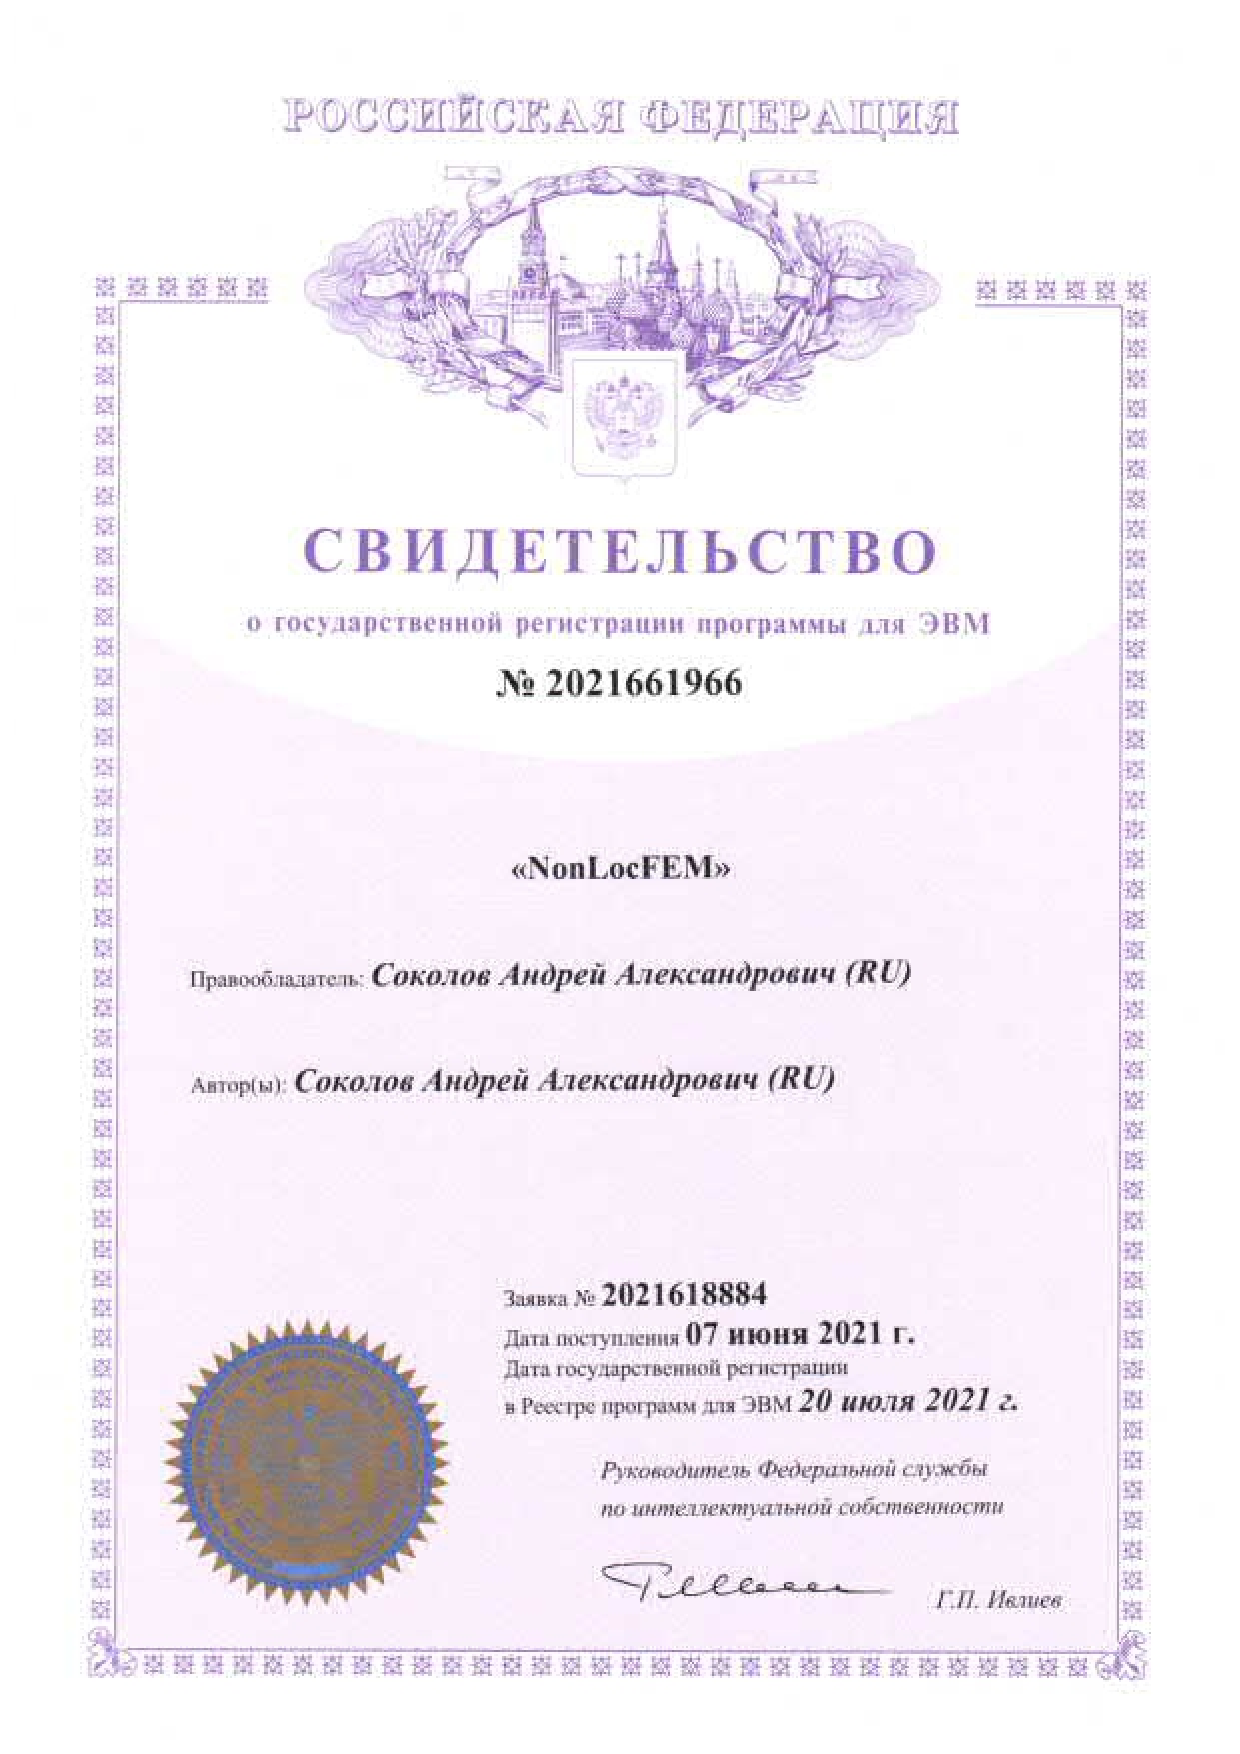
\includegraphics[height=0.65\textheight]{pics/Registration.pdf}
        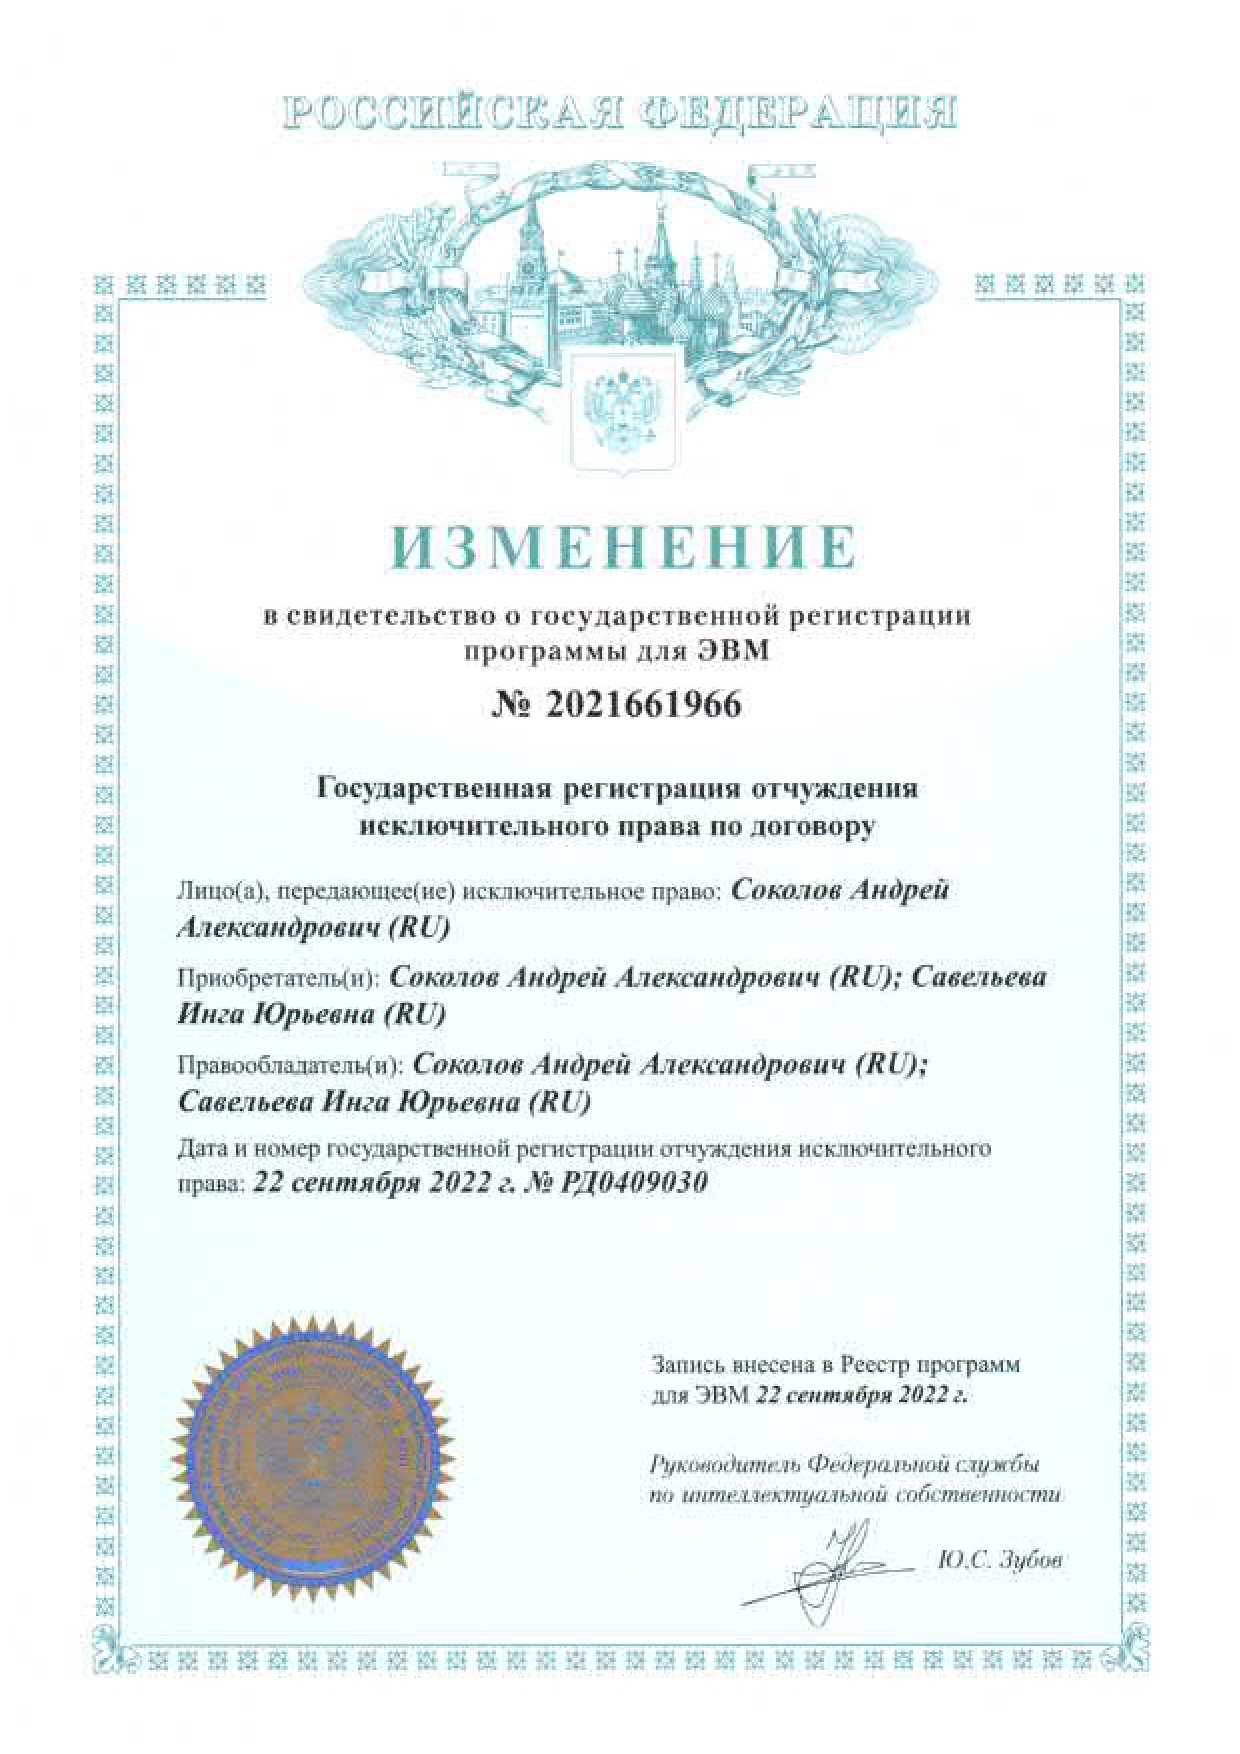
\includegraphics[height=0.65\textheight]{pics/RegistrationChange.pdf}
    \end{figure}
    
    Свидетельство о государственной регистрации программы для ЭВМ \\
    №2021661966. NonLocFEM / А. А. Соколов, И. Ю. Савельева. Зарегистрировано в Реестре программ для ЭВМ 20.07.2021.
\end{frame}

\subsection{Участие в конференциях}
\begin{frame}{Участие в конференциях}
    \begin{itemize}
    \justifying
        \item Международная научно-техническая конференция <<Актуальные проблемы прикладной математики, информатикии и механики>> (Воронеж, 2019, 2021);
        \item Международная конференция <<International Conference of Nume\-rical Analysis and Applied Mathematics>> (Родос, Греция, 2021);
        \item Международная научная конференция <<Фундаментальные и Прикладные Задачи Механики>> (Москва, 2021);
        \item Всероссийская конференция по численным методам решения задач теории упругости и пластичности (Красноярск, 2023);
        \item Международная конференция <<Математическое моделирование, численные методы и инженерное программное обеспечение>> (Москва, 2023).
    \end{itemize}
\end{frame}

\subsection{Участие в грантах}
\begin{frame}{Участие в грантах}
    \begin{itemize}
    \justifying
        \item 0705-2020-0047 <<Теория дифференциальных уравнений, краевые задачи, связанные задачи анализа и теории приближений и некоторые их приложения>>.
	\item FSFN-2023-0012 <<Разработка математических моделей и методов проектирования изделий ракетно-космической техники из перспективных конструкционных и функциональных материалов>>.
	\item FSFN-2024-0004 <<Разработка математических моделей и методов проектирования изделий ракетно-космической техники из перспективных конструкционных и функциональных материалов>>.
    \end{itemize}
\end{frame}

\begin{frame}[plain, noframenumbering] % последний слайд без оформления
    \begin{center}
        \Huge
        Спасибо за внимание!
    \end{center}
\end{frame}
